\documentclass[10pt, aspectratio=169]{beamer}
\usefonttheme{professionalfonts}
%\usetheme{CambridgeUS}
%
% Choose how your presentation looks.
%
% For more themes, color themes and font themes, see:
% http://deic.uab.es/~iblanes/beamer_gallery/index_by_theme.html
%
\mode<presentation>
{
  \usetheme{default}      % or try Darmstadt, Madrid, Warsaw, ...
  \usecolortheme{beaver} % or try albatross, beaver, crane, ...
  \usefonttheme{default}  % or try serif, structurebold, ...
  \setbeamertemplate{navigation symbols}{}
  \setbeamertemplate{caption}[numbered]
} 

\usepackage[english]{babel}
\usepackage[utf8x]{inputenc}
\usepackage{tikz}
\usepackage{pgfplots}
\usepackage{array}  % for table column M
\usepackage{makecell} % to break line within a cell
\usepackage{verbatim}
\usepackage{graphicx}
\usepackage{subcaption}
\usepackage{amsfonts}
\usepackage{amsmath}
\usepackage{bm}
\usepackage{epstopdf}
\captionsetup{compatibility=false}
%\usepackage{dsfont}
\usepackage[absolute,overlay]{textpos}
\usetikzlibrary{calc}
\usetikzlibrary{pgfplots.fillbetween, backgrounds}
\usetikzlibrary{positioning}

\usetikzlibrary{pgfplots.groupplots}
\usetikzlibrary{plotmarks}
\usetikzlibrary{calc}

\usepgfplotslibrary{groupplots}
\pgfplotsset{compat=newest} 
%\pgfplotsset{plot coordinates/math parser=false}

\usepackage{hyperref}
\hypersetup{
    colorlinks=true,
    linkcolor=blue,
    filecolor=magenta,      
    urlcolor=cyan,
}

%% 
% \def\EXTERNALIZE{1} % for externalizing figures
%%% Page numbering
\usepackage{etoolbox} % necessary for excluding beamer-only frames from page numbering

\makeatletter
\pretocmd{\beamer@@@@frame}{\alt<#1>{}{\beamer@noframenumberingtrue}}{}{}
\makeatother

\addtobeamertemplate{navigation symbols}{}{%
	\usebeamerfont{footline}%
	\usebeamercolor[fg]{footline}%
	\hspace{1em}%
	\insertframenumber/\inserttotalframenumber
}
%%%

\definecolor{matlabcomment}{RGB}{34,139,34}

\pgfmathdeclarefunction{gauss}{1}{%
	\pgfmathparse{1/(sqrt(2*pi))*exp(-((#1)^2)/2)}%
}

\pgfmathdeclarefunction{laplacian}{2}{%
	\pgfmathparse{1/(#2*2)*exp(-(abs(x-#1))/(#2))}%
}

\pgfmathdeclarefunction{pretty_func}{1}{%
	\pgfmathparse{cos(deg(#1/2)) - sin(deg(#1)) + cos(deg(#1/2)-45) - sin(deg(#1/4)-154)}%
}

\pgfplotsset{
	dirac/.style={
		mark=triangle*,
		mark options={scale=2},
		ycomb,
		scatter,
		visualization depends on={y/abs(y)-1 \as \sign},
		scatter/@pre marker code/.code={\scope[rotate=90*\sign,yshift=-2pt]}
	}
}

\def\thickness{very thick}

\tikzset{
amark/.style 2 args={
	decoration={             
		markings, 
		mark=at position {0.5} with { 
			\arrow{stealth},
			\node[#2] {#1};
		}
	}, \thickness,
	postaction={decorate}
},
earlymark/.style 2 args={
	decoration={             
		markings, 
		mark=at position {0.25} with { 
			\arrow{stealth},
			\node[#2] {#1};
		}
	}, \thickness,
	postaction={decorate}
},
latemark/.style 2 args={
	decoration={             
		markings, 
		mark=at position {0.8} with { 
			\arrow{stealth},
			\node[#2] {#1};
		}
	}, \thickness,
	postaction={decorate}
},
zpath/.style={
	decoration={             
		markings, 
		mark=at position {0.5} with { 
			\arrow{stealth},
			\node[#1] {$z^{-1}$};
		}
	}, \thickness,
	postaction={decorate}
},
terminal/.style 2 args={draw,circle,inner sep=2pt,label={#1:#2}},
}


\tikzset{
	invisible/.style={opacity=0},
	visible on/.style={alt={#1{}{invisible}}},
	alt/.code args={<#1>#2#3}{%
		\alt<#1>{\pgfkeysalso{#2}}{\pgfkeysalso{#3}} % \pgfkeysalso doesn't change the path
	},
}

\newcommand\PlotSampledSpectrum[4]{%
	\def\fs{#2}%
	\def\fmax{#3}%
	\def\ros{#4}%
	\input{#1}%
}

\pgfmathdeclarefunction{invgauss}{2}{%
	\pgfmathparse{sqrt(-2*ln(#1))*cos(deg(2*pi*#2))}%
}

\tikzset{
	declare function={
		sinc(\x) = (and(\x!=0, 1) * (sin(deg(pi*\x))/(pi*\x)) +
		(and(\x==0, 1) * 1);
	}
}

\DeclareMathOperator{\E}{\mathbb{E}} % expectation

\newcolumntype{M}[1]{>{\centering\arraybackslash}m{#1}}

\definecolor{blue2}{RGB}{51, 105, 232}  
\definecolor{red2}{RGB}{213, 15, 37}  
\definecolor{green2}{RGB}{0, 153, 37}  
\definecolor{green3}{rgb}{0.1922, 0.6392, 0.3294}% 
\definecolor{yellow2}{RGB}{238, 178, 17} 
\definecolor{gray2}{RGB}{102, 102, 102}
\definecolor{orange2}{RGB}{230, 85, 13}

% Qualitative pallete set1 from www.ColorBrewer.org
\definecolor{Qred}{RGB}{228,26,28}
\definecolor{Qblue}{RGB}{55,126,184}
\definecolor{Qgreen}{RGB}{77,175,74}
\definecolor{Qpurple}{RGB}{152,78,163}
\definecolor{Qorange}{RGB}{255,127,0}
\definecolor{Qyellow}{RGB}{255,255,51}
\definecolor{Qbrown}{RGB}{166,86,40}
\definecolor{Qpink}{RGB}{247,129,191}
\definecolor{Qgray}{RGB}{153,153,153}

\newcommand\SimpleSys[4]{%
	\def\xin{#2}%
	\def\Hz{#3}%
	\def\yout{#4}
	\input{#1}%
}

%%
\title[EE 264]{Adaptive Signal Processing}
\author{Jose Krause Perin}
\institute{Stanford University}
\date{August 6, 2018}

\begin{document}

\begin{frame}
  \titlepage
\end{frame}

\begin{frame}{Announcements}
	\begin{itemize}
		\item Thank you for the feedback on the teaching evaluation
		\item Logistics for next lectures
		\vspace{0.2cm}
		\begin{center}
			\begin{tabular}{c|c|l|c}
				\hline
				Date & Lecture	& Lecture Topic	& Reading \\
				\hline
				6-Aug	& 10 & 	Adaptive signal processing &  \\
				8-Aug	& 11 & 	The discrete Fourier transform (DFT) & 8.1--8.7 \\
				\hline
				13-Aug	& 12 & 	Spectrum analysis with the DFT	& 10.1--10.6 \\
				15-Aug	& 13 & 	Review and conclusions & \\
				\hline
			\end{tabular}
		\end{center}
		\vspace{0.2cm}
		\item HW6 will be assigned today and covers primarily lectures 10 and 11
		\item You can choose to take the final exam on either 8/16 or 8/17
	\end{itemize}
\end{frame}

\begin{frame}{Outline}
\tableofcontents
\end{frame}

%
\section{Theory}
\subsection{The adaptive linear combiner and its performance surface}
\begin{frame}{The adaptive linear combiner}

\begin{center}
%	\begin{tikzpicture}
%		\node(pic) {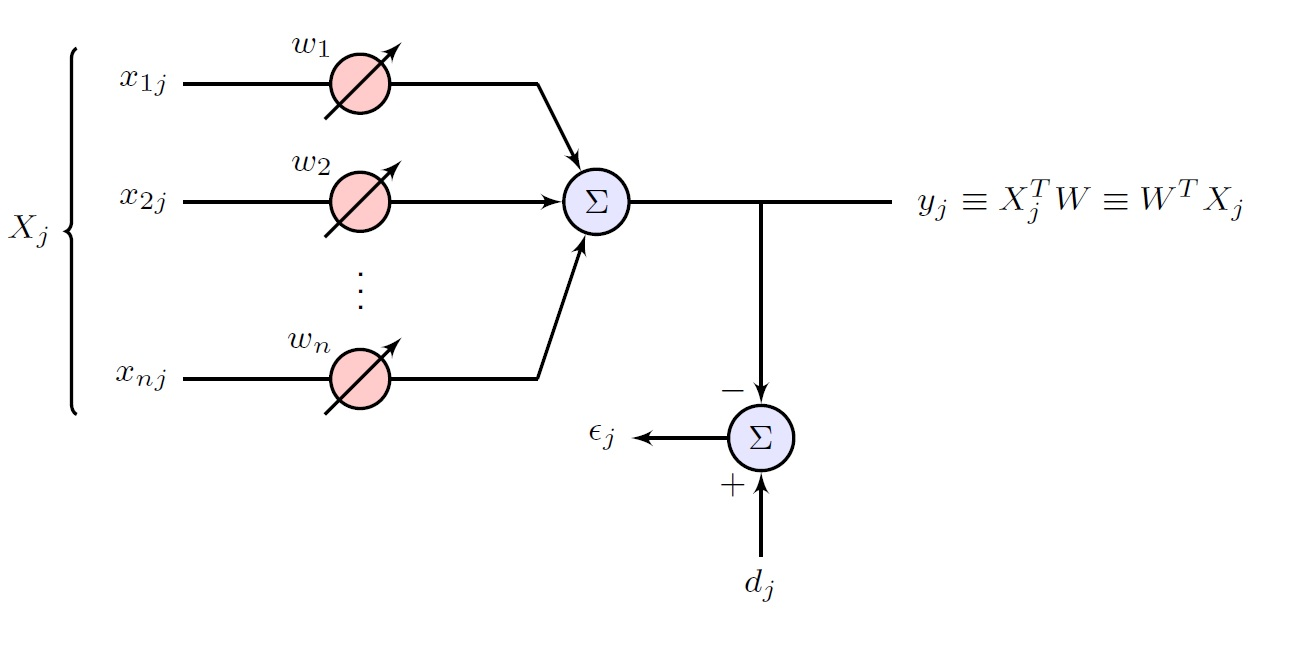
\includegraphics[width=0.7\textwidth]{figs/linear_combiner.jpg}};
%		\node[anchor=east, text width=1cm, align=center, scale=0.75] at ($(pic.west)+(0, 0.7cm)$) {Input vector};
%		\node[anchor=west, text width=1cm, align=center, scale=0.75] at ($(pic.east)+(-0.5cm, 1cm)$) {Output};
%		\node[anchor=north, text width=1.5cm, align=center, scale=0.75] at ($(pic.south)+(1.5cm, 1cm)$) {Desired response};
%		\node[anchor=south, text width=1.5cm, align=center, scale=0.75] at ($(pic.north)+(-2.5cm, -0.3cm)$) {Weights};
%		\node[anchor=north, text width=1.5cm, align=center, scale=0.75] at ($(pic.south)+(-0.45cm, 1.6cm)$) {Error};
%	\end{tikzpicture}
	\resizebox{0.7\textwidth}{!}{\def\layersep{0.5cm}
\def\outsep{0.7cm}
\def\dy{0.5}
\usetikzlibrary{backgrounds}

\begin{tikzpicture}[>=latex, shorten >= 0pt, draw=black!50, node distance=\layersep, font=\sffamily]
    \tikzstyle{node}=[circle,fill=black,minimum size=1.5pt,inner sep=0pt]
    \tikzstyle{weight}=[draw=black,circle,fill=none,minimum size=20pt,inner sep=0pt,scale=0.5]
    \tikzstyle{summer}=[weight,scale=1.8, minimum size=10pt, inner sep=2pt, scale=0.75]
    \tikzstyle{sigmoid}=[draw=black,rectangle,fill=none,minimum size=20pt,inner sep=0pt]
    \tikzstyle{annot} = [scale=0.5]

	\node[summer] (Adder) at (3*\layersep,-\dy*2.5 cm) {\large $\Sigma$}; 
    \node[node, inner sep=0pt] (mid) at (5*\layersep,-\dy*2.5 cm) {}; 
    \coordinate (output) at (7*\layersep,-\dy*2.5 cm) {};
    \node[summer, minimum size=10pt, scale=1] (error) at (5*\layersep,-\dy*5 cm) {$\Sigma$}; 
    \node[node, inner sep=0pt] (dk) at (7*\layersep,-\dy*5 cm) {};
    \coordinate[left of=error] (error-out) {};
    
    %\coordinate (A) at (\layersep,-6*\dy cm) {};
    %\coordinate (B) at (\layersep,0 cm) {};
    %\path[->] (A) edge (B);
    \draw[->] (error) -- (error-out);
    %\path[-] (error-out) edge (A);
        
    \foreach \name / \y in {1,...,3} {
    % This is the same as writing \foreach \name / \y in {1/1,2/2,3/3,4/4}
        \node[node] (I-\name) at (0,-\dy*\y) {}; % Draw the input layer nodes
        \node[weight,fill=white] (W-\name) at (\layersep,-\dy*\y cm) {$w_{\name}$}; % Draw the hidden layer  layer node     
     }   	

	\node[node] (I-4) at (0,-5*\dy cm) {}; % Draw the hidden layer 
	\node[weight, fill=white] (W-4) at (\layersep,-5*\dy cm) {$w_{M}$};
	
    %% Annotations
    \node[scale=0.5] at (-0.3,-\dy) {$X_{k1}$};
    \node[scale=0.5] at (-0.3,-\dy*2) {$X_{k2}$};
    \node[scale=0.5] at (-0.3,-\dy*3) {$X_{k3}$};
    \node[scale=0.5] at (-0.3,-\dy*5) {$X_{kn}$};
    \node[scale=0.5] at (-0.3,-\dy*3.75) {$\vdots$};
    
    \node[right, anchor=south west, scale=0.5] at ($(error.north)$){$-$};
    \node[right, anchor=north west, scale=0.5] at ($(error.east)$){$+$};
    \node[annot, above of=mid] {$X_k^TW$};
    \node[annot, below of=error-out] {error $\varepsilon_k$};
    \node[annot, right=0.01cm of output, text width=1.5cm, align=center] {$y_k$ \\ Output};
    \node[annot, right=0.01cm of dk, text width=2cm, align=center] {$d_k$ \\ Desired response};
    
    \foreach \name in {1,...,4} {
    		\path[->] (I-\name) edge (W-\name);
    		\begin{scope}[on background layer]
    			\draw[->, shorten >= -5pt, shorten <= -2pt] (W-\name.south west) -- (W-\name.north east);
   			\end{scope}
            %\path[->] (W-\name) edge (Adder);
            \draw[->] (W-\name) -- ++(15pt,0) -- (Adder);
     }
	
    \path[-] (Adder) edge (mid);
    \path[->] (mid) edge (error.north);
    \path[->] (mid) edge (output);
    \path[->] (dk) edge (error);
    
    \draw[-,decoration={brace,mirror,raise=5pt},decorate, thick]
   (-0.35,-0.7*\dy) -- node[annot, left=5pt, text width = 1cm, align=center] {$X_k$ input} (-0.35,-\dy*5.2);

\end{tikzpicture}}
\end{center}

We would like to \textit{tune} the weights $w_1, \ldots, w_M$ to minimize the error $\epsilon_k$ according to some performance metric.

In this lecture we will address the following questions:
\begin{enumerate}
	\item What is the best set of weights $w^\star_1, \ldots, w^\star_M$? 
	\item How to \textit{adapt} the weights $w_1, \ldots, w_M$ to approximately achieve $w^\star_1, \ldots, w^\star_M$?
\end{enumerate}

\end{frame}

%
\begin{frame}{The mean square error}

The \textbf{mean-square error (MSE)} is a convenient and sensible performance metric
\begin{align*}
\mathrm{MSE} = \xi &= \E(\varepsilon_k^2) \tag{by definition} \\
&= \E((d_k - X_k^TW)^2) \tag{as $\varepsilon_k = d_k - X_k^TW$} \\
&= \E(d^2_k) - 2\E(d_kX_k^T)W + W^T\E(X_kX_k^T)W 
\end{align*}

The MSE is a \textbf{quadratic function} of the weights. There's only one minimum.

\begin{center}
	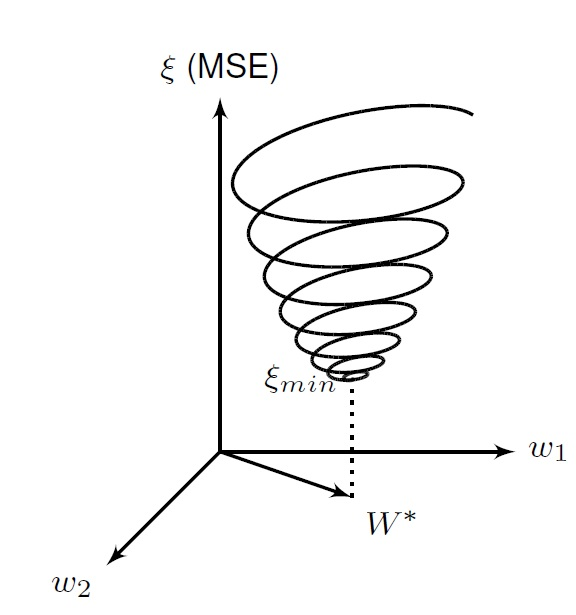
\includegraphics[width=0.32\textwidth]{figs/performance_surface.jpg}	
\end{center}

\end{frame}

\begin{frame}{The performance surface}

	\begin{align*}
	\mathrm{MSE} = \xi &= \E(d^2_k) - 2\E(d_kX_k^T)W + W^T\E(X_kX_k^T)W
	\end{align*}

	To ease the notation we make a few definitions
	\begin{align*}
	P &\equiv \E(d_kX_k) \tag{Cross-correlation between input and desired response} \\
	R &\equiv \E(X_kX_k^T) \tag{Autocorrelation matrix}
	\end{align*}
	
	More explicitly:

	\begin{equation*}
		P = \begin{bmatrix}
			\E(d_kx_{1k}) \\
			\E(d_kx_{2k}) \\
			\vdots \\
			\E(d_kx_{Mk})
		\end{bmatrix} \qquad\qquad R = \begin{bmatrix}
			\E(x_{1k}x_{1k}) & \E(x_{1k}x_{2k}) & \ldots & \E(x_{1k}x_{nk}) \\
			\E(x_{2k}x_{1k}) & \E(x_{2k}x_{2k}) & \ldots & \E(x_{2k}x_{nk}) \\
				\vdots & \vdots & \ddots & \vdots \\
			\E(x_{nk}x_{1k}) & \E(x_{nk}x_{2k}) & \ldots & \E(x_{nk}x_{nk})
		\end{bmatrix} 
	\end{equation*}
\end{frame}

\begin{frame}
	Substituting $P = \E(d_kX_k)$ and $R = \E(X_kX_k^T)$ in our equation for the MSE results in 

	\begin{align*}
		\mathrm{MSE} = \xi = \E(d^2_k) - 2P^TW + W^TRW
	\end{align*}
	
	The minimum of the quadratic function is where the first derivative is zero:
	
	\begin{align}
	\frac{d}{dW}\mathrm{MSE} = 0 \implies W^\star = R^{-1}P \tag{Wiener solution}
	\end{align}
	
	The \textbf{Wiener solution} is the set of weights $W^\star$ that minimize the MSE.
	
	\vspace{0.5cm}
	At the \textbf{Wiener solution}, the MSE is minimum
	\begin{equation}
		\mathrm{MSE}|_{W =W^{\star}} = \xi_{min} = E(d^2_k) - P^TR^{-1}P \tag{Minimum MSE}
	\end{equation}
\end{frame}

\begin{frame}{The orthogonality principle}
	
	At the Wiener solution, the error is \textbf{orthogonal} to the input.
	
	In statistical terms, the error is \textbf{uncorrelated} to the input.
	
	\begin{equation}
		\E(\varepsilon_kX_k)\Big|_{W = W^\star} = 0 \tag{orthogonality principle}
	\end{equation}
	
	This property is known as the \textbf{orthogonality principle}, and it is true for all least-squares solution.
	
\end{frame}

\begin{frame}{An FIR filter as a linear combiner}
The input to the adaptive linear combiner is $X = [x[n], x[n-1], \ldots, x[n-M+1]]^T$

\begin{center}
	\resizebox{0.8\textwidth}{!}{\def\layersep{0.5cm}
\def\outsep{0.7cm}
\def\dy{0.5}
\usetikzlibrary{backgrounds}

\begin{tikzpicture}[>=latex, shorten >= 0pt, draw=black!50, node distance=\layersep, font=\sffamily]
    \tikzstyle{node}=[circle,fill=black,minimum size=1.5pt,inner sep=0pt]
    \tikzstyle{weight}=[draw=black,circle,fill=none,minimum size=20pt,inner sep=0pt,scale=0.5]
    \tikzstyle{summer}=[weight,scale=1.8, minimum size=10pt, inner sep=2pt, scale=0.75]
    \tikzstyle{sigmoid}=[draw=black,rectangle,fill=none,minimum size=20pt,inner sep=0pt]
    \tikzstyle{annot} = [scale=0.5]

	\node[summer] (Adder) at (3*\layersep,-\dy*2.5 cm) {\large $\Sigma$}; 
    \node[node, inner sep=0pt] (mid) at (5*\layersep,-\dy*2.5 cm) {}; 
    \coordinate (output) at (7*\layersep,-\dy*2.5 cm) {};
    \node[summer, minimum size=10pt, scale=1] (error) at (5*\layersep,-\dy*5 cm) {$\Sigma$}; 
    \node[node, inner sep=0pt] (dk) at (7*\layersep,-\dy*5 cm) {};
    \coordinate[left of=error] (error-out) {};
    
    %\coordinate (A) at (\layersep,-6*\dy cm) {};
    %\coordinate (B) at (\layersep,0 cm) {};
    %\path[->] (A) edge (B);
    \draw[->] (error) -- (error-out);
    %\path[-] (error-out) edge (A);
        
    \foreach \name / \y in {1,...,3} {
    % This is the same as writing \foreach \name / \y in {1/1,2/2,3/3,4/4}
    	\node[node] (I-\name) at (0,-\dy*\y cm) {};
        \node[weight,fill=white] (W-\name) at (\layersep,-\dy*\y cm) {$w_{\name}$}; % Draw the hidden layer  layer node     
        \draw[->] (I-\name) -- (W-\name);
     } 
 	
 	\node[weight, fill=white] (W-4) at (\layersep,-5*\dy cm) {$w_{L}$};
 	\node[node] (I-4) at (0,-\dy*5 cm) {};
 	\draw[->] (I-4) -- (W-4);
 	
	\coordinate (M-1) at ($(I-1)!0.5!(I-2)$) {};  	
	\coordinate (M-2) at ($(I-2)!0.5!(I-3)$) {};
	\coordinate (M-3) at ($(I-3)!0.5!(I-4)$) {};
	
	\draw[->] (I-1) -- (M-1);
	\draw[-] (M-1) -- (I-2);
	\draw[->] (I-2) -- (M-2);
	\draw[-] (M-2) -- (I-3);
	\draw[-, dotted] (I-3) -- (I-4);
	
	\node[left=0.05cm of M-1, scale=0.5] {$z^{-1}$};
	\node[left=0.05cm of M-2, scale=0.5] {$z^{-1}$};

	

	
	
    %% Annotations
    \node[node] (x) at (-0.5,-\dy) {};
    \draw[->] (x) -- (I-1);
    \draw[->] (I-1) -- (W-1);
    \node[left=0.1cm of x, scale=0.5] {$x[n]$};
    
    \node[right, anchor=south west, scale=0.5] at ($(error.north)$){$-$};
    \node[right, anchor=north west, scale=0.5] at ($(error.east)$){$+$};
    \node[annot, above of=mid] {$x[n] \ast w[n]$};
    \node[annot, below of=error-out] {error $e[n]$};
    \node[annot, right=0.01cm of output, text width=1.5cm, align=center] {$y[n]$ \\ Output};
    \node[annot, right=0.01cm of dk, text width=2cm, align=center] {$d[n]$ \\ Desired response};
    
    \foreach \name in {1,...,4} {
    		\begin{scope}[on background layer]
    			\draw[->, shorten >= -5pt, shorten <= -2pt] (W-\name.south west) -- (W-\name.north east);
   			\end{scope}
            %\path[->] (W-\name) edge (Adder);
            \draw[->] (W-\name) -- ++(15pt,0) -- (Adder);
     }
	
    \path[-] (Adder) edge (mid);
    \path[->] (mid) edge (error.north);
    \path[->] (mid) edge (output);
    \path[->] (dk) edge (error);

\end{tikzpicture}}
\end{center}

The resulting FIR filter has coefficients $\{w_1, \ldots, w_M\}$.

\end{frame}

\begin{frame}

The optimal filter coefficients are given by the Wiener solution
\begin{equation*}
	W^{\star} = R^{-1}P
\end{equation*}

And we can compute the vector $P$ and matrix $R$ as we did before
\begin{equation*}
	P = \begin{bmatrix}
		\E(d[n]x[n]) \\
		\E(d[n]x[n-1]) \\
		\vdots \\
		\E(d[n]x_[n-N])
	\end{bmatrix} 
\end{equation*}

\begin{equation*}
	R = \begin{bmatrix}
		\E(x[n]x[n]) & \E(x[n]x[n-1]) & \ldots & \E(x[n]x[n-N]) \\
		\E(x[n-1]x[n]) & \E(x[n-1]x[n-1]) & \ldots & \E(x[n-1]x[n-N]) \\
		\vdots & \vdots & \ddots & \vdots \\
		\E(x[n-N]x[n]) & \E(x[n-N]x[n-1]) & \ldots & \E(x[n-N]x[n-N]) \\
	\end{bmatrix} 
\end{equation*}
\end{frame}

\begin{frame}
	Recall that the autocorrelation function is defined by
	\begin{equation*}
		\phi_{xx}[m] = \E(x[n+m]x^*[n])
	\end{equation*}

	Now we're just writing it in matrix form
	\begin{equation*}
		R = \begin{bmatrix}
				\phi_{xx}[0] & \phi_{xx}[1] & \ldots & \phi_{xx}[N] \\
				\phi_{xx}[1] & \phi_{xx}[0] & \ldots & \phi_{xx}[N-1] \\
				\vdots & \vdots & \ddots & \vdots \\
				\phi_{xx}[N] & \phi_{xx}[N-1] & \ldots & \phi_{xx}[0] \\
		\end{bmatrix} 
	\end{equation*}
	
	In Matlab: \\
	\noindent\texttt{>> phi\_xx = xcorr(x, x, N)} \\
	\noindent\texttt{>> R = toeplitz(phi\_xx(N+1:end))}
\end{frame}

\subsection{Adaptation algorithms}
\frame{\tableofcontents[currentsubsection]}

\begin{frame}{Adaptation algorithms}
\begin{center}
	\resizebox{0.7\textwidth}{!}{\def\layersep{0.5cm}
\def\outsep{0.7cm}
\def\dy{0.5}
\usetikzlibrary{backgrounds}

\begin{tikzpicture}[>=latex, shorten >= 0pt, draw=black!50, node distance=\layersep, font=\sffamily]
    \tikzstyle{node}=[circle,fill=black,minimum size=1.5pt,inner sep=0pt]
    \tikzstyle{weight}=[draw=black,circle,fill=none,minimum size=20pt,inner sep=0pt,scale=0.5]
    \tikzstyle{summer}=[weight,scale=1.8, minimum size=10pt, inner sep=2pt, scale=0.75]
    \tikzstyle{sigmoid}=[draw=black,rectangle,fill=none,minimum size=20pt,inner sep=0pt]
    \tikzstyle{annot} = [scale=0.5]

	\node[summer] (Adder) at (3*\layersep,-\dy*2.5 cm) {\large $\Sigma$}; 
    \node[node, inner sep=0pt] (mid) at (5*\layersep,-\dy*2.5 cm) {}; 
    \coordinate (output) at (7*\layersep,-\dy*2.5 cm) {};
    \node[summer, minimum size=10pt, scale=1] (error) at (5*\layersep,-\dy*5 cm) {$\Sigma$}; 
    \node[node, inner sep=0pt] (dk) at (7*\layersep,-\dy*5 cm) {};
    \coordinate[left of=error] (error-out) {};
    
    %\coordinate (A) at (\layersep,-6*\dy cm) {};
    %\coordinate (B) at (\layersep,0 cm) {};
    %\path[->] (A) edge (B);
    \draw[->] (error) -- (error-out);
    %\path[-] (error-out) edge (A);
        
    \foreach \name / \y in {1,...,3} {
    % This is the same as writing \foreach \name / \y in {1/1,2/2,3/3,4/4}
    	\node[node] (I-\name) at (0,-\dy*\y cm) {};
        \node[weight,fill=white] (W-\name) at (\layersep,-\dy*\y cm) {$w_{\name}$}; % Draw the hidden layer  layer node     
        \draw[->] (I-\name) -- (W-\name);
     } 
 	
 	\node[weight, fill=white] (W-4) at (\layersep,-5*\dy cm) {$w_{L}$};
 	\node[node] (I-4) at (0,-\dy*5 cm) {};
 	\draw[->] (I-4) -- (W-4);
 	
	\coordinate (M-1) at ($(I-1)!0.5!(I-2)$) {};  	
	\coordinate (M-2) at ($(I-2)!0.5!(I-3)$) {};
	\coordinate (M-3) at ($(I-3)!0.5!(I-4)$) {};
	
	\draw[->] (I-1) -- (M-1);
	\draw[-] (M-1) -- (I-2);
	\draw[->] (I-2) -- (M-2);
	\draw[-] (M-2) -- (I-3);
	\draw[-, dotted] (I-3) -- (I-4);
	
	\node[left=0.05cm of M-1, scale=0.5] {$z^{-1}$};
	\node[left=0.05cm of M-2, scale=0.5] {$z^{-1}$};

	

	
	
    %% Annotations
    \node[node] (x) at (-0.5,-\dy) {};
    \draw[->] (x) -- (I-1);
    \draw[->] (I-1) -- (W-1);
    \node[left=0.1cm of x, scale=0.5] {$x[n]$};
    
    \node[right, anchor=south west, scale=0.5] at ($(error.north)$){$-$};
    \node[right, anchor=north west, scale=0.5] at ($(error.east)$){$+$};
    \node[annot, above of=mid] {$x[n] \ast w[n]$};
    \node[annot, below of=error-out] {error $e[n]$};
    \node[annot, right=0.01cm of output, text width=1.5cm, align=center] {$y[n]$ \\ Output};
    \node[annot, right=0.01cm of dk, text width=2cm, align=center] {$d[n]$ \\ Desired response};
    
    \foreach \name in {1,...,4} {
    		\begin{scope}[on background layer]
    			\draw[->, shorten >= -5pt, shorten <= -2pt] (W-\name.south west) -- (W-\name.north east);
   			\end{scope}
            %\path[->] (W-\name) edge (Adder);
            \draw[->] (W-\name) -- ++(15pt,0) -- (Adder);
     }
	
    \path[-] (Adder) edge (mid);
    \path[->] (mid) edge (error.north);
    \path[->] (mid) edge (output);
    \path[->] (dk) edge (error);

\end{tikzpicture}}
\end{center}

\textbf{Problem:} We know that $W^\star = R^{-1}P$, but in practice, $R$ and $P$ are either unknown or hard to compute/estimate. How can we find some $W$ such that $W \approx W^\star$? 

\begin{enumerate}
	\item Newton's method
	\item Steepest descent
	\item The \textbf{least-mean squares (LMS)} algorithm
\end{enumerate}

\end{frame}

\begin{frame}{Adaptation algorithms: Newton's method}
	\begin{equation*}
		W \leftarrow W - \mu R^{-1}\nabla \tag{adaptation equation}
	\end{equation*}
	where $\mu$ is the adaptation constant, and $\nabla$ is the gradient of the MSE, i.e., $\nabla \equiv \frac{\partial}{\partial W}\mathrm{MSE}$.
	
	\begin{center}
		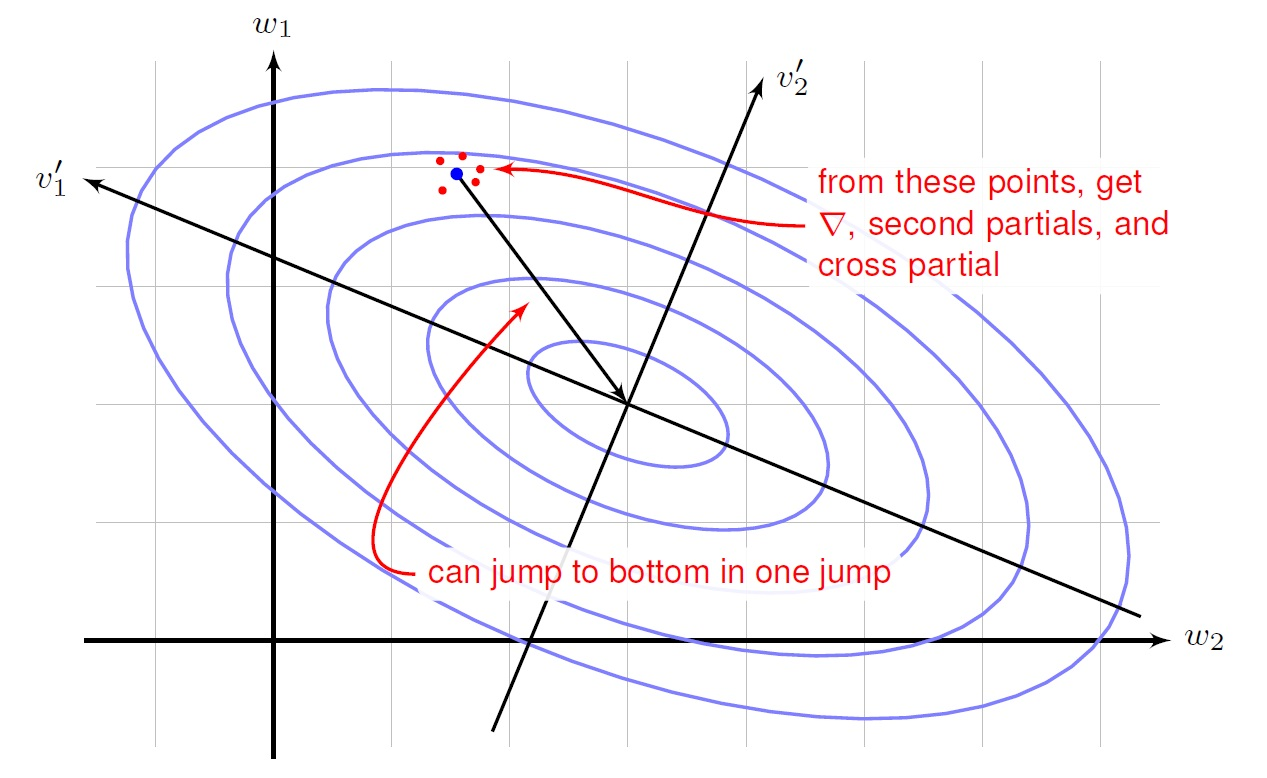
\includegraphics[width=0.5\textwidth]{figs/newton_method.jpg}	
	\end{center}
	
	 $R^{-1}$ scales and directs the step to $W^\star$. Convergence happens in one step!
	 
	 \textbf{Problem:} requires knowledge of $R$ and $\nabla$.
 	
\end{frame}

\begin{frame}{Adaptation algorithms: steepest descent}
\begin{equation*}
W \leftarrow W - \mu \nabla \tag{adaptation equation}
\end{equation*}

\begin{center}
	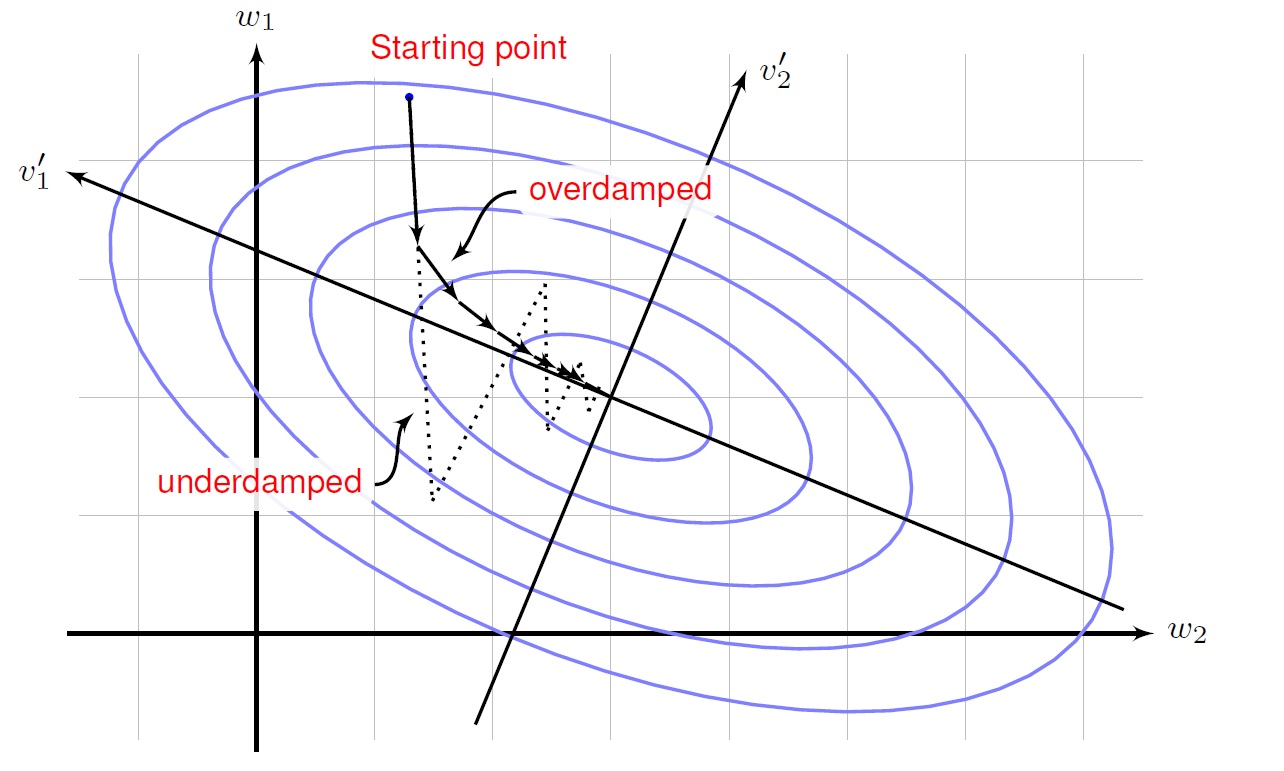
\includegraphics[width=0.5\textwidth]{figs/steepest_descent.jpg}	
\end{center}

\begin{itemize}
	\item $W$ is adapted in the direction of \textbf{steepest descent} of the gradient
	
	\item Must estimate the gradient $\nabla$ somehow.
\end{itemize}


\end{frame}

%
\begin{frame}{Adaptation algorithms: the LMS algorithm}

The \textbf{least mean squares (LMS)} algorithm is a form of steepest descent where the gradient is estimated from the \textbf{instantaneous error}

\begin{equation}
	\varepsilon_n^2 = (d_n - X_n^TW)^2 \tag{instantaneous error}
\end{equation}

\begin{equation}
	\hat{\nabla} = \frac{\partial \varepsilon_n}{\partial W} = 2(d_n - X_n^TW)X_n = 2\varepsilon_nX_n \tag{gradient estimate}
\end{equation}

\begin{equation*}
W \leftarrow W + 2\mu e_nX_n \tag{LMS weight update}
\end{equation*}

Gradient estimate is very noisy, but on average the weights \textit{generally} move to the Wiener solution.
\end{frame}

%
\begin{frame}{Adaptation algorithms: the LMS algorithm}

The LMS algorithm: \\
\begin{tabular}{l}
	\hline
	Initialize the weights to some value $W \leftarrow W_0$ \\
	\textbf{For} each input and desired response pair ($X_n$, $d_n$): \\
	\qquad Compute the output $y_n = X_n^TW$ \\
	\qquad Compute the instantaneous error $e_n = (d_n - y_n)$ \\
	\qquad Update the weights: $W \leftarrow W + 2\mu e_nX_n$ \\
	\textbf{end} \\
	\hline 
\end{tabular}

If $X$ is complex, then the adaptation equation changes slightly $W \leftarrow W + 2\mu e_nX_n^*$.
\end{frame}

%
\begin{frame}{Learning curve}
\begin{itemize}
	\item The learning curve is a plot of the average MSE $\E(e^2_n)$ over time.
	\item To obtain an empirical learning curve, we run the LMS algorithm $N$ times with different weight initializations.
	\item For each run, we obtain a MSE curve $\mathrm{MSE}^{(1)}, \ldots, \mathrm{MSE}^{(N)}$ i.e., $\mathrm{MSE}^{(i)} = e_n^2$.
	\item Then we average the result
	\begin{equation}
	\E(\xi_k^2) \approx \frac{\mathrm{MSE}^{(1)}+ \ldots+ \mathrm{MSE}^{(N)}}{N}
	\end{equation}

	\item The learning curve is a sum of decaying exponentials with time constants 
		\begin{align*}
		(\tau_{MSE})_n &\approx \frac{1}{4\mu\lambda_n}~\text{iterations} \tag{Steepest descent \& LMS} 
	\end{align*}
	where $\lambda_n$ is the $n$th eigenvalue of matrix $R$.	
\end{itemize}
\end{frame}

\begin{frame}{Learning curve}
Example of learning curve
\begin{center}
	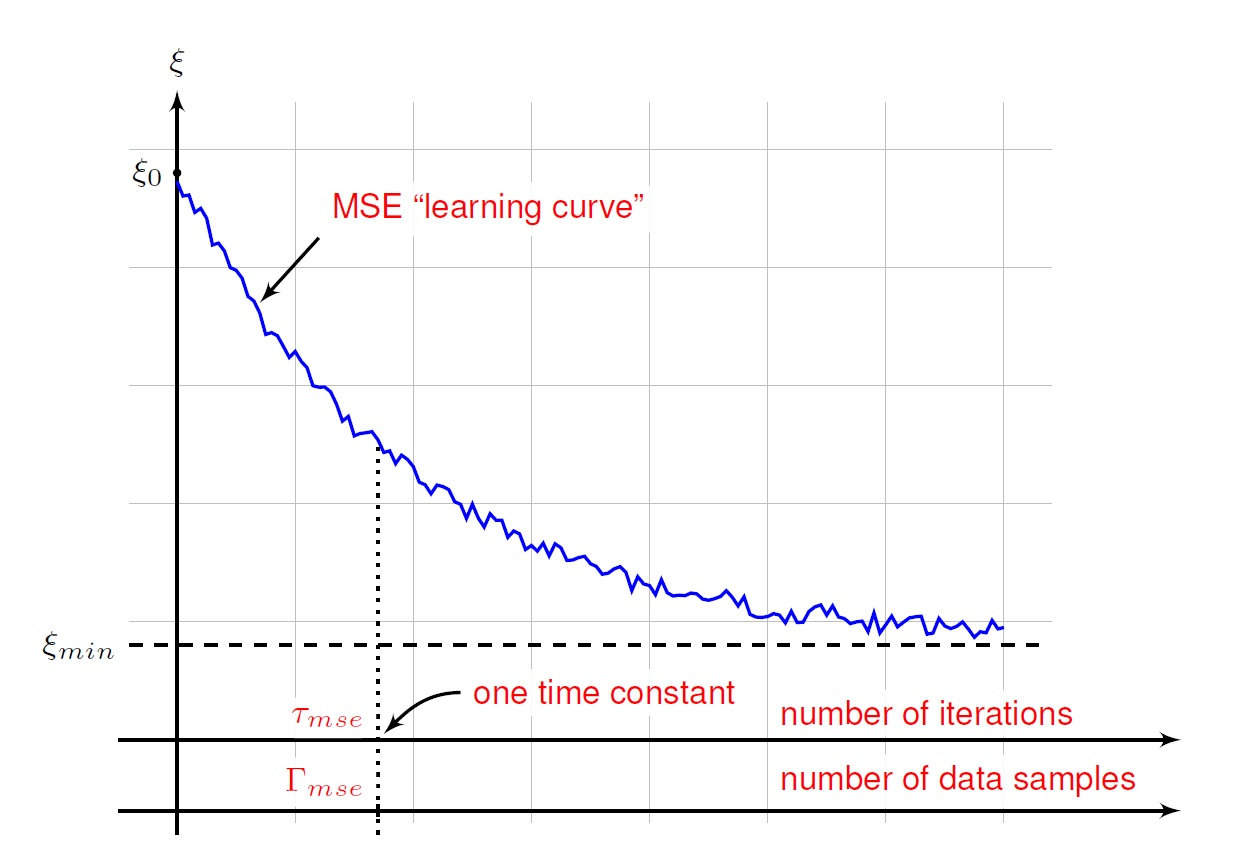
\includegraphics[width=0.75\textwidth]{figs/learning_curve.jpg}
\end{center}
\end{frame}

%
\begin{frame}{Stability of the LMS algorithm}

\begin{itemize}
	\item The constant $\mu > 0$ is known as the \textbf{adaptation constant}.
	\item If $\mu$ is too small, the algorithm will take too long to converge (small steps).
	\item If $\mu$ is too large, the algorithm can become unstable. 
	\item It can be shown that stability is guarantee if
	\begin{equation}
	0 < \mu < \frac{1}{\mathrm{trace} R} \tag{stability condition} 
	\end{equation}
	where $\mathrm{trace}$ is the sum of all elements in the main diagonal of a matrix.
	\item When applying the LMS algorithm to determine the coefficients of an $M$th-order FIR filter we have that $\mathrm{trace} R = (M+1)\phi_{xx}[0]$. 
\end{itemize}
\end{frame}

\begin{frame}{Excess noise and misadjustment}
	Error in the gradient estimate leads to excess MSE
	\begin{center}
		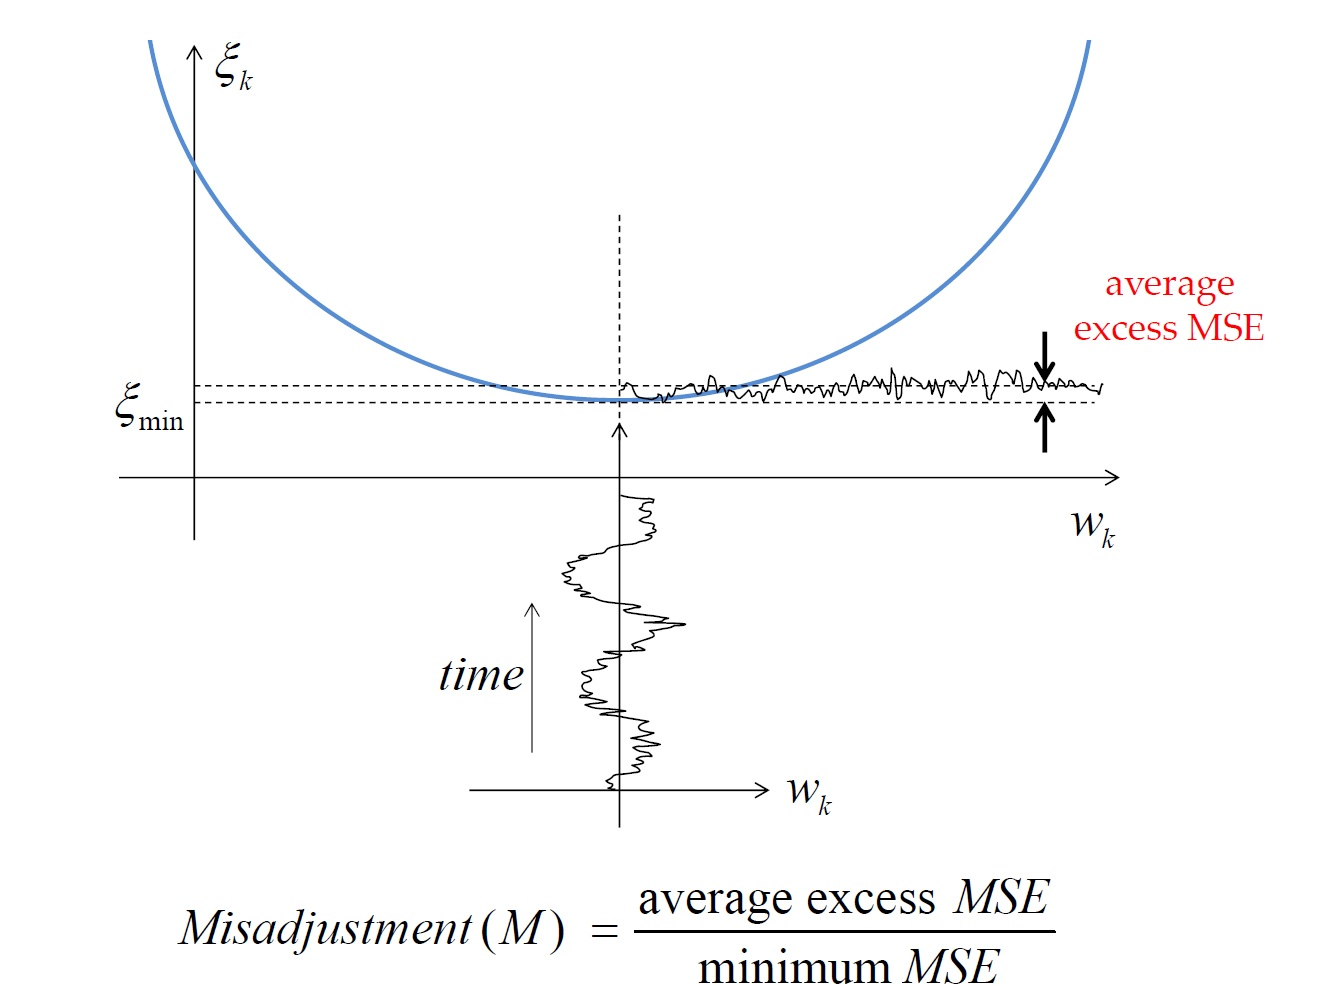
\includegraphics[width=0.5\textwidth, trim=0cm 2cm 0cm 0cm, clip]{figs/misadjustment.jpg}	
	\end{center}
	\begin{equation}
		\text{Misadjustment} = \frac{\text{excess noise}}{\text{minimum MSE}}\tag{definition}
	\end{equation}
	
	For the LMS algorithm:
	\begin{equation*}
		M = \mu\mathrm{trace}(R)
	\end{equation*}	
\end{frame}

\begin{frame}{Performance metrics}
	
	\begin{block}{Parameters to tune}
		\begin{itemize}
			\item Number of weights
			\item Adaptation constant $\mu$
		\end{itemize}
	\end{block}

	\begin{block}{What to look for}
		\begin{itemize}
			\item Minimum MSE: is the number of weights high enough?
			\item Time constants: how fast will the adaptive algorithm reach the minimum MSE?
			\item Excess MSE or misadjustment: how oscillatory are the solutions produced by the adaptive algorithm near the optimal solution?
		\end{itemize}
	\end{block}
\end{frame}


\section{Application examples}
\frame{\tableofcontents[currentsection]}

\subsection{Linear equalization}
\begin{frame}{Linear equalization with decision-directed learning}
\centering
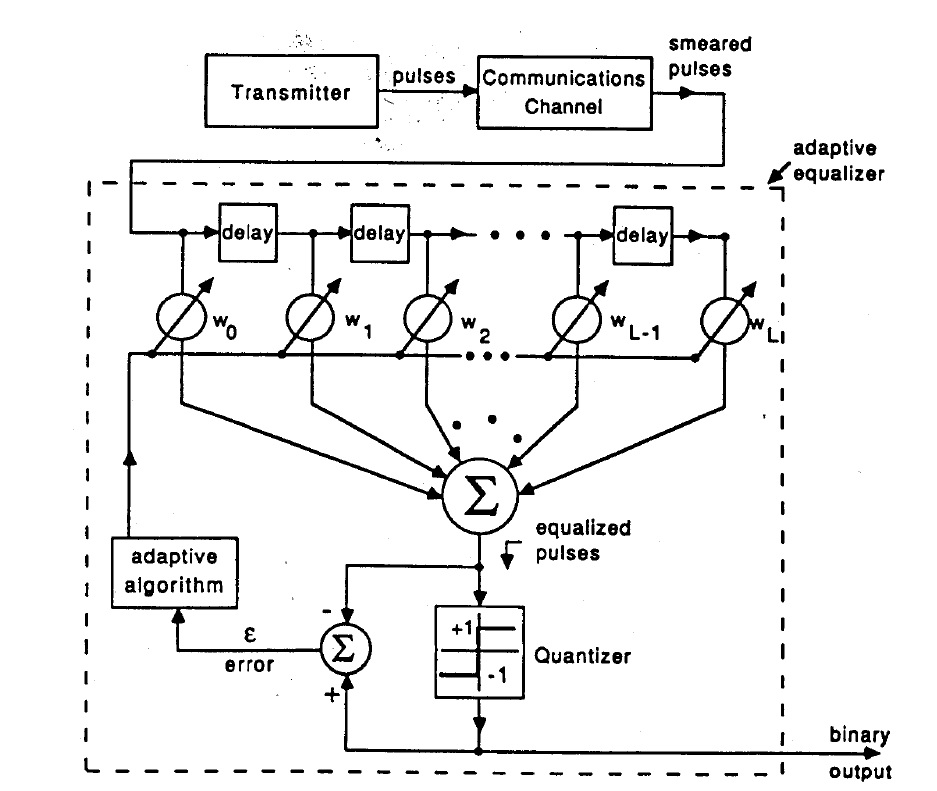
\includegraphics[width=0.6\textwidth]{figs/equalizer.jpg}
\end{frame}

\begin{frame}{Eye diagram before and after equalization}
	\begin{figure}
		\centering
		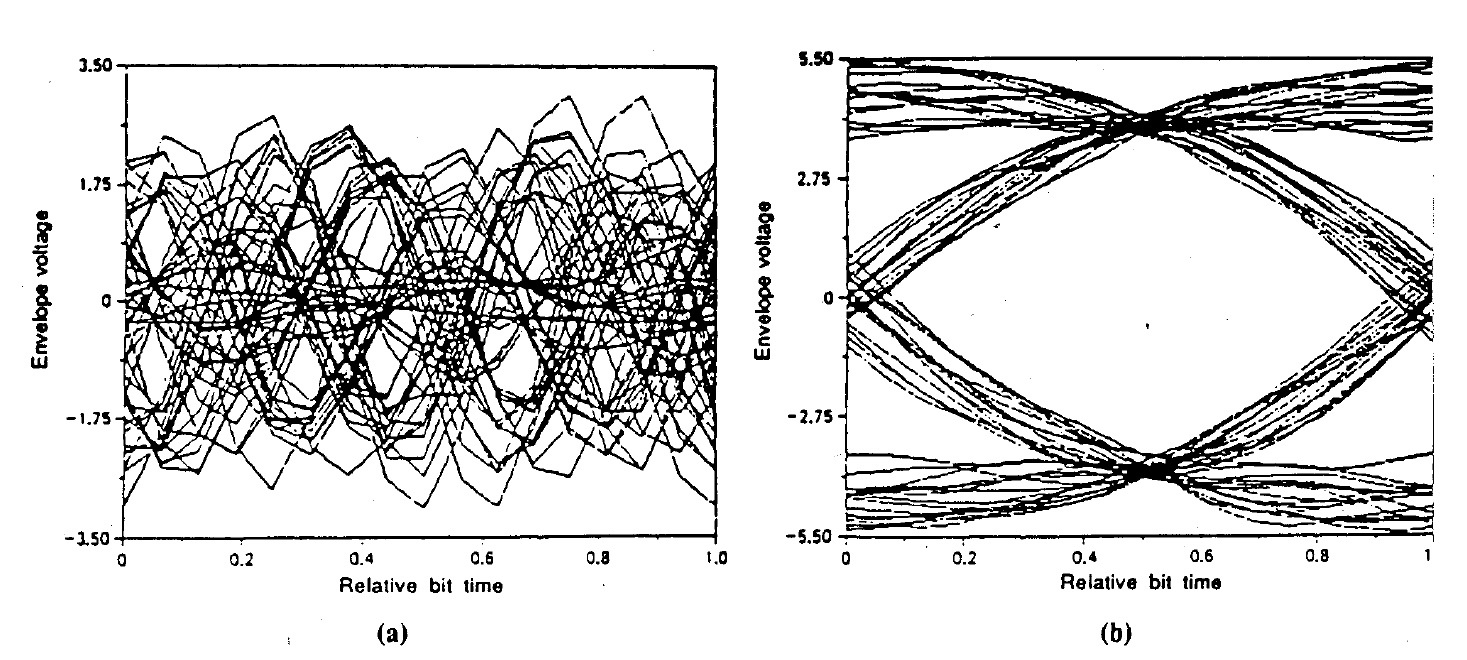
\includegraphics[width=\textwidth]{figs/eye-diagram.jpg}
		\caption{(a) Before and (b) after equalization.}
	\end{figure}
\end{frame}

\subsection{Noise canceling}
\frame{\tableofcontents[currentsubsection]}
\begin{frame}{Noise canceling}
	\begin{figure}
		\centering
		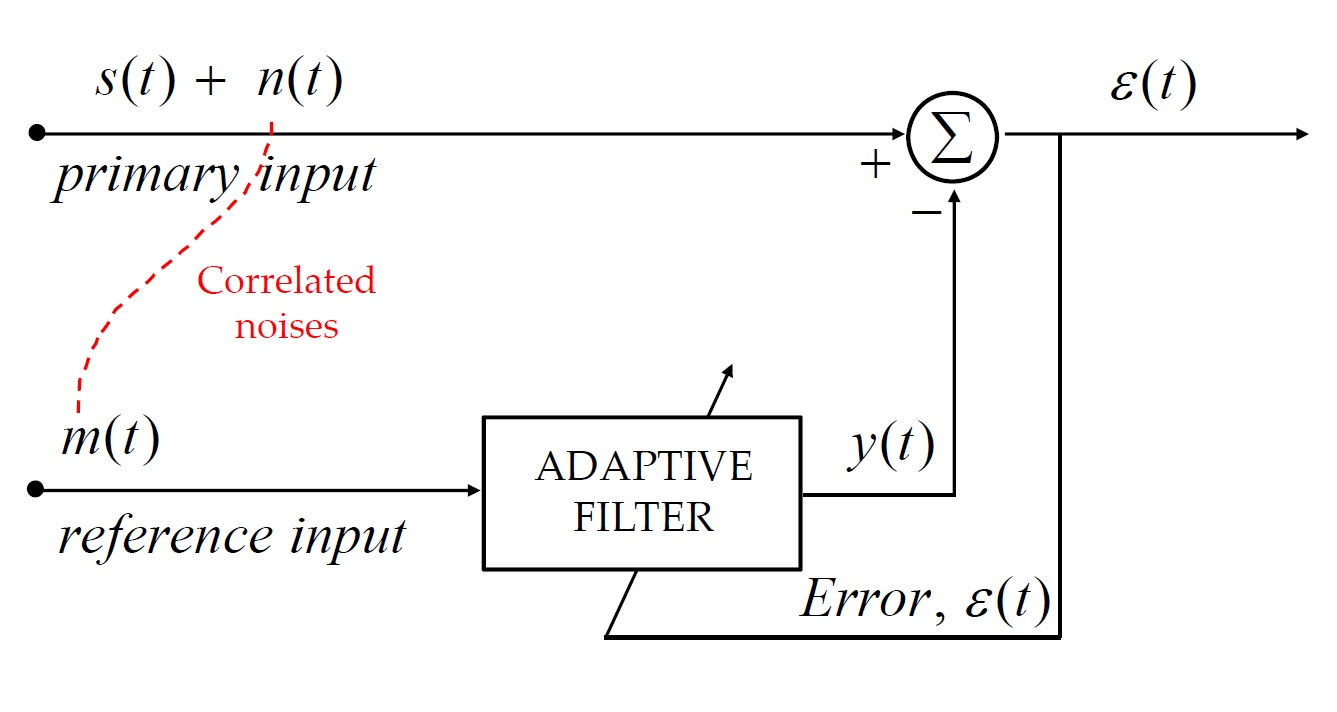
\includegraphics[width=0.8\textwidth, trim=0cm 1cm 0cm 0cm, clip]{figs/noise_canceling.jpg}
	\end{figure}
	\begin{align}
		\varepsilon &= s + n - y \tag{error} \\
		\E(\varepsilon^2) &= \E((s + n - y)^2) \tag{Mean square error} \\
		&= \E(s^2) + \E((n - y)^2) \tag{$\E(s(n-y)) = 0$ from assumption}
	\end{align}
	
	\begin{itemize}
		\item Minimizing the error $\E(\varepsilon^2)$ is equivalent to minimizing $\E((n - y)^2)$ 
		\item After adaptation, $y \approx n$ and $\varepsilon \approx s$ (approximated in the least squares sense).
	\end{itemize} 
\end{frame}

\begin{frame}{Examples of noise canceling applications}
Canceling 60Hz interference from biological signals. 
\begin{center}
	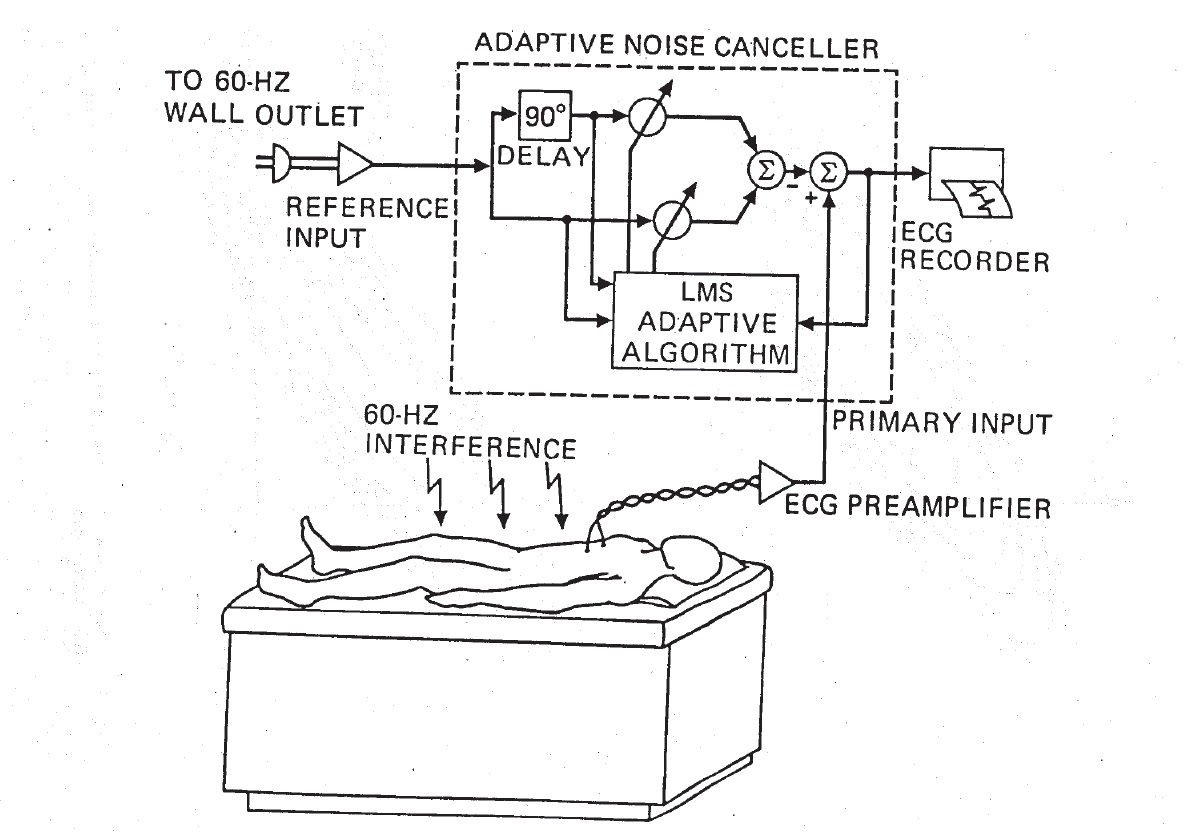
\includegraphics[width=0.7\textwidth]{figs/60Hz_interference.jpg}
\end{center}

\end{frame}

\begin{frame}{Examples of noise canceling applications}
\begin{center}
	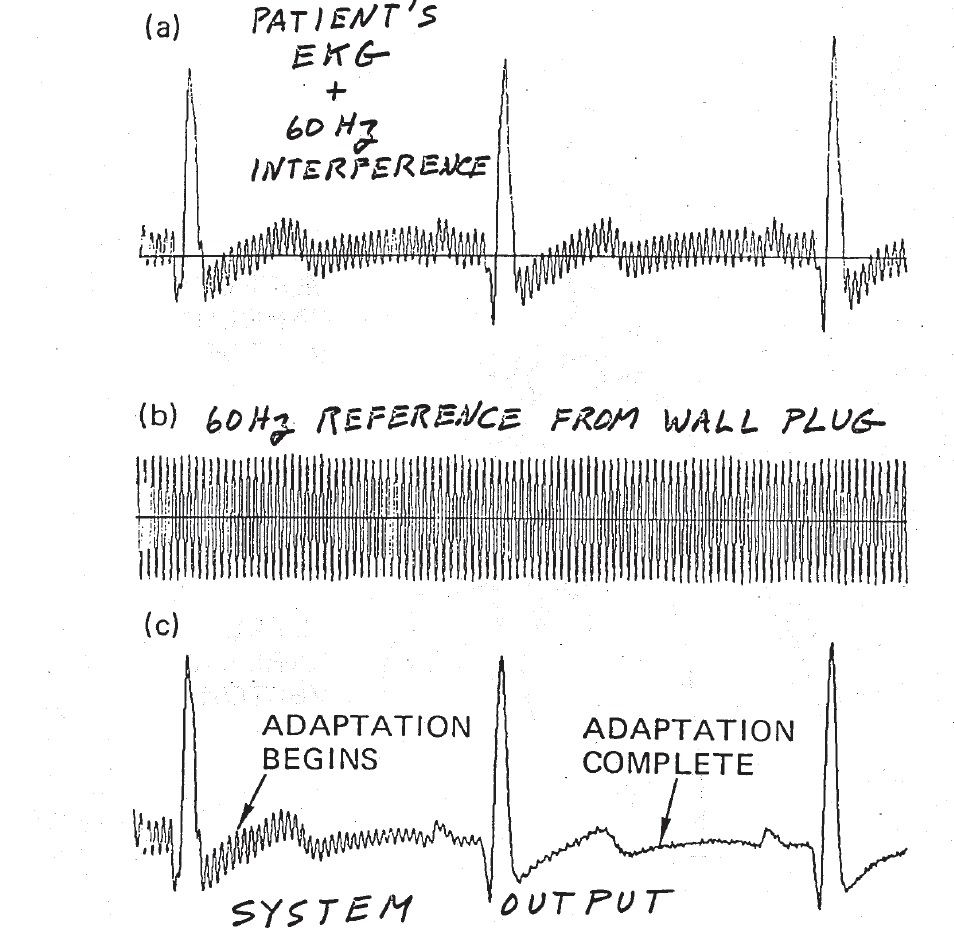
\includegraphics[width=0.5\textwidth]{figs/60Hz_interference_cancel.jpg}
\end{center}

\end{frame}


\subsection{Inverse control}
\frame{\tableofcontents[currentsubsection]}
\begin{frame}{Inverse control}
\begin{itemize}
	\item In control problems we would like to make a plant (a system) respond to a given command and produce a desired output (e.g., setting the room temperature, controlling the blood pressure of a patient, etc)
	
	\begin{center}
		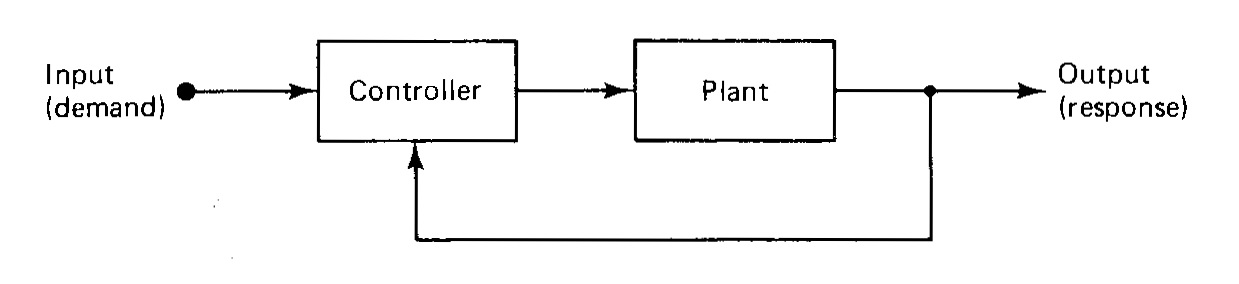
\includegraphics[width=\textwidth]{figs/control.jpg}
	\end{center}
	
	\item We use adaptive filters for two basic operations in control problems
	\begin{itemize}
		\item \normalsize Plant identification
		\item \normalsize Plant inversion
	\end{itemize}
\end{itemize}
\end{frame}

\begin{frame}{Basic operations: plant identification}
	The adaptive filter models the plant
	\begin{center}
		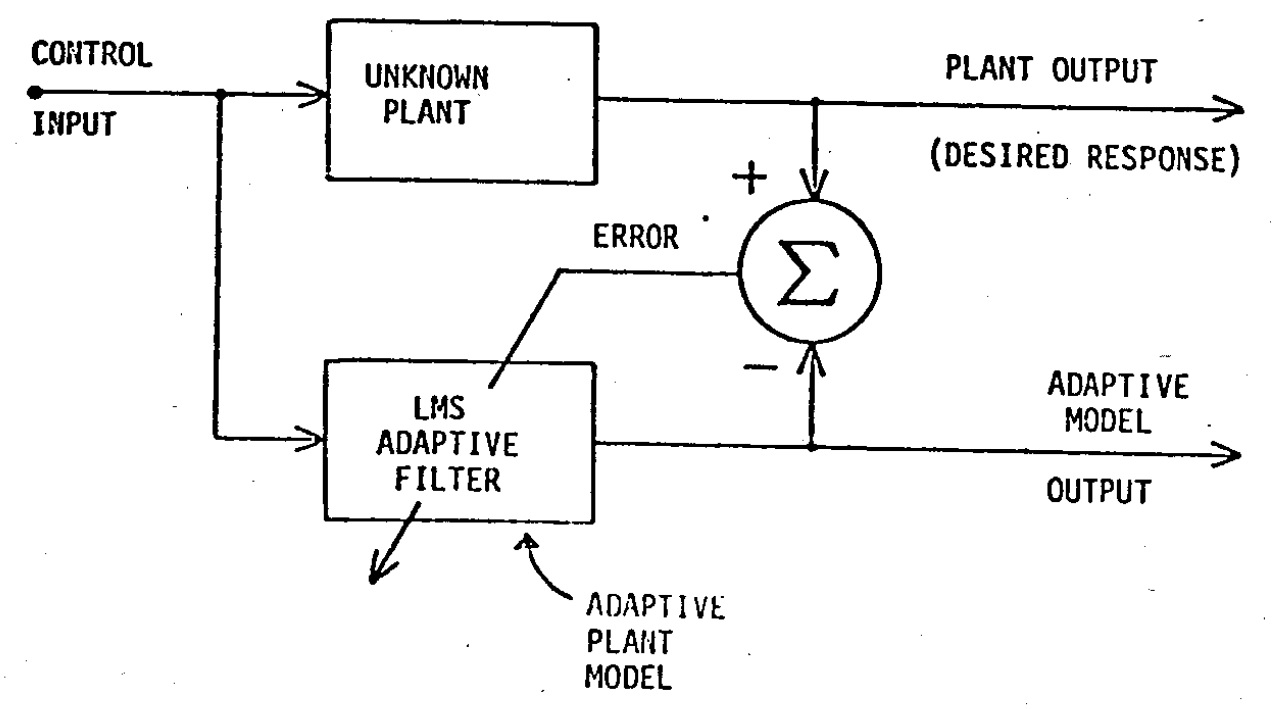
\includegraphics[width=0.7\textwidth, angle=1]{figs/plant_id.jpg}
	\end{center}
\end{frame}


\begin{frame}{Basic operations: plant inverse}
The adaptive filter models the inverse of the plant
\begin{center}
	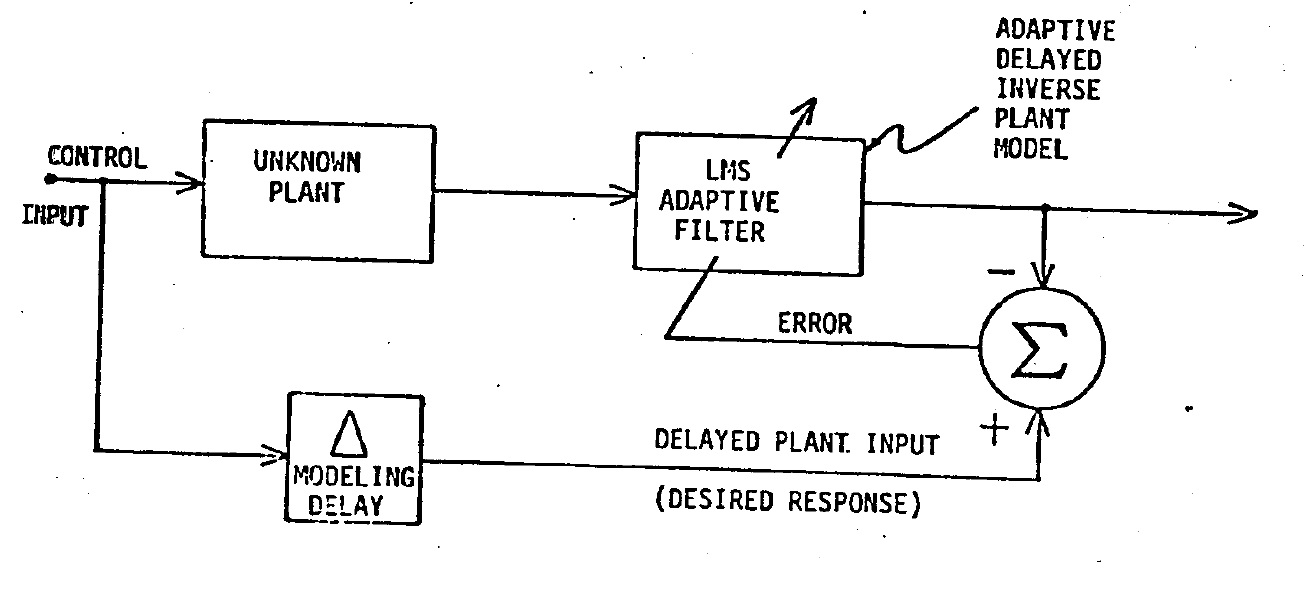
\includegraphics[width=0.6\textwidth, angle=1.5, trim=0cm 1.5cm 1.5cm 0cm, clip]{figs/inverse_control.jpg}
\end{center}
We need to consider what happens if the plant is \textbf{non-minimum phase}. That is, if it has zeros outside the unit circle (unstable inverse).
\begin{itemize}
	\item For any discrete-time system $H(z)$, we can write $H(z) = H_{min}(z)H_{ap}(z)$, where $H_{min}(z)$ is a minimum phase system, and $H_{ap}(z)$ is an all-pass system.
	\item The adaptive filter will converge to $H_{min}^{-1}(z)$, and it'll not compensate for phase distortion (and delay) due to $H_{ap}(z)$.
\end{itemize}
\end{frame}

\begin{frame}{Summary}
	\begin{itemize}
		\item The linear combiner is the basis of adaptive systems and adaptive filtering
		\item We use the mean square error (MSE) as the performance metric
		\item The Wiener solution is the optimal set of weights that minimizes the MSE
		\item The LMS algorithm is a simple way to train the adaptive filter to approximate the Wiener solution
		\item The LMS algorithm uses the instantaneous error to obtain an estimate of the gradient
		\item This estimate is very noisy, but on average it converges to the Wiener solution
		\item We adjust the adaption constant to control how fast the LMS algorithm converges and how noisy the solutions near the Wiener solution (excess noise and misadjustment)
	\end{itemize}
\end{frame}

%
\end{document}
